\documentclass[tikz]{standalone}

\usepackage{tikz}
\usetikzlibrary{cd}

\begin{document}

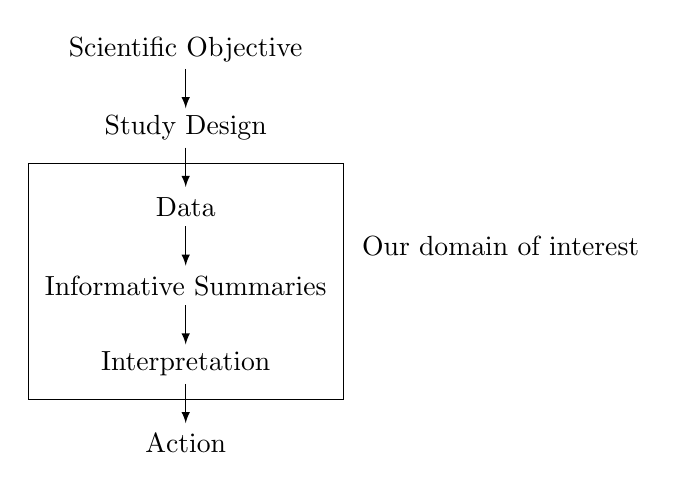
\begin{tikzpicture}

\node at (0,0) {Scientific Objective};
\node at (0,-1) {Study Design};
\node at (0,-2) {Data};
\node at (0,-3) {Informative Summaries};
\node at (0,-4) {Interpretation};
\node at (0,-5) {Action};

\draw [-latex] (0,-.25) -- (0,-.75);
\draw [-latex] (0,-1.25) -- (0,-1.75);
\draw [-latex] (0,-2.25) -- (0,-2.75);
\draw [-latex] (0,-3.25) -- (0,-3.75);
\draw [-latex] (0,-4.25) -- (0,-4.75);

\draw [rectangle] (-2,-1.45) -- (2,-1.45) -- (2,-4.45) -- (-2, -4.45) -- (-2,-1.45);

\node at (4, -2.5) {Our domain of interest};
\end{tikzpicture}
\end{document}